\section{Role Constellations in Sustainability Transitions}
\label{sec:role-constellations}

\subsection{Conceptual Foundations}

Sustainability transitions research has historically prioritized structural-systemic analyses, with the Multi-Level Perspective (MLP) serving as the dominant framework \citep{geels2002technological}. However, scholars note that transition research ``lacks a suitable vocabulary to analyse the (changing) interactions and relations of actors'' \citep[p.~45]{wittmayer2017actor}. While agency is acknowledged as integral to transitions \citep{geels2011multi}, the operationalization of actor interactions remains limited.

\textbf{Role constellations} refer to relational configurations among actor roles---patterns of cooperation, competition, and mutual influence shaping transition dynamics. Following \citet{wittmayer2017actor}, we define \textit{roles} as recognizable sets of activities addressing recurring situations, and \textit{transition roles} as those through which actors support or hinder specific transitions. Related terminology includes \textit{actor constellations} \citep{kriesi2001swiss}, \textit{actor configurations} \citep{avelino2016shifting}, and \textit{practice constellations} \citep{shove2012dynamics}.

\subsection{Theoretical Frameworks}

The Multi-Actor Perspective (MaP) distinguishes four institutional sectors (state, market, third sector, community) and three aggregation levels (sectors, organizations, individuals), with a hybrid sphere of boundary-crossing intermediaries \citep{avelino2016shifting}. \citet{wittmayer2017actor} operationalized sociological role theory for transitions, identifying constellation dynamics including cooperative, antagonistic, and independent relationships.

\citet{bodenheimer2021lost} linked roles to transition phases via the Dialectic Issue Lifecycle Model, showing how constellations evolve from problem emergence (issue identifiers vs.\ status quo maintainers) through political debate (coalition builders, framers) to stabilization (institutional integrators). Key typologies distinguish niche actors (innovation champions, frontrunners) from regime actors, now recognized as heterogeneous \citep{kungl2025incumbent}. Intermediary typologies identify systemic, regime-based, niche, process, and user intermediaries \citep{kivimaa2019typology}.

\subsection{Research Gaps}

\begin{table}[htbp]
\centering
\small
\caption{Research gaps in role constellation scholarship}
\label{tab:gaps}
\begin{tabular}{@{}p{2.8cm}p{5.2cm}@{}}
\toprule
\textbf{Gap Type} & \textbf{Description} \\
\midrule
Weak theorization & Constellations invoked but rarely operationalized \\
Static analysis & Snapshots dominate; evolution understudied \\
Cross-level integration & Individual--organizational--systemic levels disconnected \\
Geographic bias & Global South underrepresented \\
Sectoral imbalance & Energy dominates; agri-food, buildings neglected \\
Incumbent heterogeneity & Limited differentiation among incumbent types \\
Multi-system dynamics & Cross-sector interactions poorly understood \\
\bottomrule
\end{tabular}
\end{table}

Despite significant field growth \citep{kohler2019agenda}, explicit constellation theorization remains underdeveloped. Most studies capture static configurations rather than tracking evolution across phases. Integration across micro (psychology), meso (organizations), and macro (institutions) levels is limited \citep{upham2019thinking}. Non-human agency is largely neglected despite material-discursive turns \citep{contesse2021unravelling}. Empirically, Global South contexts remain underrepresented, energy transitions dominate sectoral coverage, and multi-system interactions require further investigation.

\subsection{Research Opportunities}

We identify seven priority directions for advancing role constellation research:

\begin{enumerate}[noitemsep,topsep=0pt]
    \item \textbf{Systematic typology development}: Classify constellation patterns (cooperative, competitive, hybrid, emergent) beyond ad hoc descriptions.
    \item \textbf{Longitudinal studies}: Track constellation evolution across transition phases, identifying tipping points and reconfiguration moments.
    \item \textbf{Multi-scale integration}: Bridge psychological micro-foundations with organizational dynamics and institutional conditioning.
    \item \textbf{Incumbent peripheral actors}: Investigate how actors from adjacent regimes (banks, universities, regulators) shape transitions \citep{coen2025view}.
    \item \textbf{Comparative cross-context analysis}: Systematic comparison across sectors, regions, and governance scales.
    \item \textbf{Methodological pluralism}: Combine network analysis, computational text methods, and participatory approaches.
    \item \textbf{Governance applications}: Develop actionable constellation diagnostics for policymakers and transition managers.
\end{enumerate}

A ``constellation turn'' complementing the established niche-regime-landscape focus with systematic attention to relational configurations could significantly advance both theoretical understanding and practical governance of sustainability transitions.


% Preamble requirements:
% \usepackage{tikz}
% \usetikzlibrary{positioning,shapes,arrows.meta,calc,backgrounds,fit,decorations.pathmorphing}

%% ============================================
%% FIGURE 1: Multi-Actor Perspective (Sectors)
%% ============================================
\begin{figure}[htbp]
\centering
\begin{tikzpicture}[
    sector/.style={circle, minimum size=2.8cm, draw, thick, fill=#1!15},
    hybrid/.style={ellipse, minimum width=1.8cm, minimum height=1cm, draw, dashed, fill=gray!10},
    lbl/.style={font=\small\bfseries},
    scale=0.9
]
% Four sectors as overlapping circles
\node[sector=blue] (state) at (0,1.8) {};
\node[lbl] at (0,1.8) {State};
\node[sector=orange] (market) at (1.8,0) {};
\node[lbl] at (1.8,0) {Market};
\node[sector=green!70!black] (community) at (0,-1.8) {};
\node[lbl] at (0,-1.8) {Community};
\node[sector=purple] (third) at (-1.8,0) {};
\node[lbl] at (-1.8,0) {Third Sector};

% Hybrid sphere in center
\node[hybrid] (hyb) at (0,0) {\scriptsize Hybrid};

% Axis labels
\node[font=\scriptsize, anchor=south] at (0,3.2) {\textit{Public}};
\node[font=\scriptsize, anchor=north] at (0,-3.2) {\textit{Private}};
\node[font=\scriptsize, anchor=west] at (3.2,0) {\textit{For-profit}};
\node[font=\scriptsize, anchor=east] at (-3.2,0) {\textit{Non-profit}};
\end{tikzpicture}
\caption{Multi-Actor Perspective: Four institutional sectors}
\label{fig:map-sectors}
\end{figure}

%% ============================================
%% FIGURE 2: Role Constellation Dynamics
%% ============================================
\begin{figure}[htbp]
\centering
\begin{tikzpicture}[
    role/.style={circle, draw, thick, minimum size=1.1cm, fill=#1!20, font=\scriptsize},
    coop/.style={-Stealth, thick, green!60!black},
    antag/.style={-Stealth, thick, red!70!black, dashed},
    influence/.style={-Stealth, gray, thick},
    mutual/.style={Stealth-Stealth, blue!60, thick},
    scale=0.95
]
% Niche roles (left cluster)
\node[role=teal] (innov) at (-3,1.5) {Innovator};
\node[role=teal] (champ) at (-3,-0.5) {Champion};
\node[role=teal] (early) at (-1.5,0.5) {Early\\Adopter};

% Regime roles (right cluster)  
\node[role=orange] (incumb) at (3,1) {Incumbent};
\node[role=orange] (resist) at (3,-1) {Resistor};
\node[role=orange] (adapt) at (1.5,0) {Adapter};

% Intermediary (center)
\node[role=purple] (inter) at (0,2.2) {Intermediary};

% Audience (bottom)
\node[role=gray] (aud) at (0,-2) {Audience};

% Cooperative links (niche)
\draw[coop] (innov) -- (champ);
\draw[coop] (champ) -- (early);
\draw[coop] (innov) to[bend left=20] (early);

% Antagonistic links
\draw[antag] (champ) -- (resist);
\draw[antag] (early) -- (incumb);

% Mutual influence
\draw[mutual] (inter) -- (innov);
\draw[mutual] (inter) -- (incumb);
\draw[mutual] (adapt) -- (early);

% Influence on audience
\draw[influence] (champ) -- (aud);
\draw[influence] (resist) -- (aud);
\draw[influence] (inter) to[bend right=30] (aud);

% Legend
\matrix[anchor=north west, font=\scriptsize] at (-4.5,-2.8) {
    \draw[coop] (0,0) -- (0.6,0); & \node{Cooperative}; \\
    \draw[antag] (0,0) -- (0.6,0); & \node{Antagonistic}; \\
    \draw[mutual] (0,0) -- (0.6,0); & \node{Mutual influence}; \\
};
\end{tikzpicture}
\caption{Role constellation dynamics: cooperation, antagonism, and influence}
\label{fig:constellation-dynamics}
\end{figure}

%% ============================================
%% FIGURE 3: Phase-Constellation Evolution
%% ============================================
\begin{figure}[htbp]
\centering
\begin{tikzpicture}[
    phase/.style={rectangle, rounded corners, draw, thick, minimum width=2cm, minimum height=3.5cm, fill=#1!8},
    role/.style={circle, draw, minimum size=0.5cm, fill=#1!40, inner sep=1pt, font=\tiny},
    arr/.style={-Stealth, thick, gray},
    timeline/.style={-Stealth, very thick},
    scale=0.75
]
% Timeline arrow
\draw[timeline] (-0.5,-2.5) -- (14,-2.5) node[anchor=west]{\small Time};

% Phase boxes
\node[phase=red!30] (p1) at (1,0.5) {};
\node[anchor=north, font=\scriptsize\bfseries] at (1,2.5) {Emergence};

\node[phase=orange!30] (p2) at (4,0.5) {};
\node[anchor=north, font=\scriptsize\bfseries] at (4,2.5) {Rising\\Concerns};

\node[phase=yellow!50] (p3) at (7,0.5) {};
\node[anchor=north, font=\scriptsize\bfseries] at (7,2.5) {Political\\Debate};

\node[phase=green!30] (p4) at (10,0.5) {};
\node[anchor=north, font=\scriptsize\bfseries] at (10,2.5) {Policy\\Formation};

\node[phase=blue!20] (p5) at (13,0.5) {};
\node[anchor=north, font=\scriptsize\bfseries] at (13,2.5) {Stabilization};

% Phase 1 roles
\node[role=teal] at (0.6,1.2) {I};
\node[role=teal] at (1.4,0.8) {A};
\node[role=gray] at (1,0) {S};

% Phase 2 roles (more, connected)
\node[role=teal] (r2a) at (3.5,1.5) {I};
\node[role=teal] (r2b) at (4.5,1.3) {C};
\node[role=teal] (r2c) at (4,0.5) {E};
\node[role=orange] (r2d) at (4,-0.5) {R};
\draw[thin,gray] (r2a)--(r2b)--(r2c);

% Phase 3 roles (complex)
\node[role=teal] (r3a) at (6.5,1.5) {F};
\node[role=purple] (r3b) at (7.5,1.5) {B};
\node[role=teal] (r3c) at (6.5,0.3) {M};
\node[role=orange] (r3d) at (7.5,0.3) {H};
\node[role=orange] (r3e) at (7,-0.7) {R};
\draw[thin,green!50!black] (r3a)--(r3b);
\draw[thin,red!50] (r3c)--(r3d);
\draw[thin,gray] (r3b)--(r3c);

% Phase 4 roles
\node[role=purple] (r4a) at (9.5,1.5) {L};
\node[role=blue!70] (r4b) at (10.5,1.5) {P};
\node[role=orange] (r4c) at (9.5,0.3) {A};
\node[role=teal] (r4d) at (10.5,0.3) {D};
\node[role=gray] (r4e) at (10,-0.7) {U};
\draw[thin,blue] (r4a)--(r4b);
\draw[thin,green!50!black] (r4c)--(r4d);

% Phase 5 roles (integrated)
\node[role=blue!70] (r5a) at (12.5,1.2) {I};
\node[role=green!60!black] (r5b) at (13.5,1.2) {S};
\node[role=green!60!black] (r5c) at (13,0) {D};
\draw[thin,green!50!black] (r5a)--(r5b)--(r5c)--(r5a);

% Arrows between phases
\foreach \i/\j in {1/4, 4/7, 7/10, 10/13} {
    \draw[arr] (\i+1.3,0.5) -- (\j-1.3,0.5);
}

% Legend
\node[anchor=north west, font=\tiny] at (-0.5,-3.2) {
    I=Identifier, A=Attention, S=Status quo, C=Champion, E=Early adopter, R=Resistor,
    F=Framer, B=Broker, M=Market dev., H=Hedger, L=Lobbyist, P=Policymaker, D=Demand, U=User
};
\end{tikzpicture}
\caption{Role constellation evolution across transition phases}
\label{fig:phase-evolution}
\end{figure}

%% ============================================
%% FIGURE 4: Niche-Regime Constellation Network
%% ============================================
\begin{figure}[htbp]
\centering
\begin{tikzpicture}[
    niche/.style={circle, draw=teal, thick, fill=teal!15, minimum size=0.9cm, font=\tiny},
    regime/.style={circle, draw=orange!80!black, thick, fill=orange!15, minimum size=0.9cm, font=\tiny},
    intermed/.style={diamond, draw=purple, thick, fill=purple!15, minimum size=0.8cm, font=\tiny, inner sep=0pt},
    landscape/.style={rectangle, rounded corners, draw=gray, dashed, fill=gray!5},
    strong/.style={-, very thick},
    weak/.style={-, thin, gray},
    conflict/.style={-, thick, red!60, decorate, decoration={zigzag, segment length=4, amplitude=1}},
    scale=0.85
]
% Background regions
\begin{scope}[on background layer]
    \node[landscape, minimum width=4cm, minimum height=5cm] at (-2.5,0) {};
    \node[landscape, minimum width=4cm, minimum height=5cm, fill=orange!5] at (2.5,0) {};
    \node[anchor=north, font=\scriptsize\itshape, gray] at (-2.5,2.8) {Niche space};
    \node[anchor=north, font=\scriptsize\itshape, gray] at (2.5,2.8) {Regime};
\end{scope}

% Niche actors
\node[niche] (n1) at (-3.5,1.5) {N1};
\node[niche] (n2) at (-2,1.8) {N2};
\node[niche] (n3) at (-3,0) {N3};
\node[niche] (n4) at (-1.5,0.3) {N4};
\node[niche] (n5) at (-2.5,-1.5) {N5};

% Regime actors
\node[regime] (r1) at (2,1.5) {R1};
\node[regime] (r2) at (3.5,1) {R2};
\node[regime] (r3) at (2.5,-0.3) {R3};
\node[regime] (r4) at (3.8,-1) {R4};
\node[regime] (r5) at (2,-1.5) {R5};

% Intermediaries
\node[intermed] (i1) at (0,1.5) {I1};
\node[intermed] (i2) at (0,-0.8) {I2};

% Niche internal links
\draw[strong, teal!60] (n1)--(n2);
\draw[strong, teal!60] (n2)--(n4);
\draw[weak] (n3)--(n4);
\draw[weak] (n3)--(n5);
\draw[strong, teal!60] (n4)--(n5);

% Regime internal links
\draw[strong, orange!60] (r1)--(r2);
\draw[strong, orange!60] (r2)--(r3);
\draw[strong, orange!60] (r3)--(r4);
\draw[weak] (r4)--(r5);
\draw[weak] (r1)--(r3);

% Cross-boundary via intermediaries
\draw[strong, purple!60] (n2)--(i1);
\draw[strong, purple!60] (i1)--(r1);
\draw[strong, purple!60] (n4)--(i2);
\draw[strong, purple!60] (i2)--(r3);
\draw[weak] (i1)--(i2);

% Conflict links
\draw[conflict] (n4)--(r3);
\draw[conflict] (n5)--(r5);

% Legend
\matrix[anchor=north west, draw, rounded corners, fill=white, font=\tiny, inner sep=3pt] at (-4.5,-2.5) {
    \node[niche, minimum size=0.5cm]{}; & \node{Niche actor}; &
    \node[regime, minimum size=0.5cm]{}; & \node{Regime actor}; &
    \node[intermed, minimum size=0.4cm]{}; & \node{Intermediary}; \\
};
\end{tikzpicture}
\caption{Niche-regime constellation network with intermediary bridging}
\label{fig:niche-regime-network}
\end{figure}

%% ============================================
%% FIGURE 5: Constellation Typology
%% ============================================
\begin{figure}[htbp]
\centering
\begin{tikzpicture}[
    node/.style={circle, draw, thick, minimum size=0.7cm, fill=#1!25},
    box/.style={rectangle, rounded corners, draw, minimum width=3.2cm, minimum height=2.8cm},
    coop/.style={-, green!60!black, thick},
    antag/.style={-, red!60, thick, dashed},
    mixed/.style={-, blue!50, thick, dotted},
    scale=0.8
]
% Cooperative constellation
\node[box] (c1) at (0,0) {};
\node[anchor=north, font=\small\bfseries] at (0,1.6) {Cooperative};
\node[node=green!70!black] (c1a) at (-0.7,0.5) {};
\node[node=green!70!black] (c1b) at (0.7,0.5) {};
\node[node=green!70!black] (c1c) at (0,-0.7) {};
\draw[coop] (c1a)--(c1b)--(c1c)--(c1a);

% Competitive constellation
\node[box] (c2) at (4,0) {};
\node[anchor=north, font=\small\bfseries] at (4,1.6) {Competitive};
\node[node=red!70] (c2a) at (3.3,0.5) {};
\node[node=red!70] (c2b) at (4.7,0.5) {};
\node[node=red!70] (c2c) at (4,-0.7) {};
\draw[antag] (c2a)--(c2b);
\draw[antag] (c2b)--(c2c);
\draw[antag] (c2c)--(c2a);

% Hybrid constellation
\node[box] (c3) at (8,0) {};
\node[anchor=north, font=\small\bfseries] at (8,1.6) {Hybrid};
\node[node=teal] (c3a) at (7.3,0.5) {};
\node[node=orange] (c3b) at (8.7,0.5) {};
\node[node=purple] (c3c) at (8,-0.7) {};
\draw[coop] (c3a)--(c3c);
\draw[antag] (c3a)--(c3b);
\draw[mixed] (c3b)--(c3c);

% Emergent constellation
\node[box] (c4) at (12,0) {};
\node[anchor=north, font=\small\bfseries] at (12,1.6) {Emergent};
\node[node=gray] (c4a) at (11.3,0.7) {};
\node[node=gray] (c4b) at (12.7,0.5) {};
\node[node=gray] (c4c) at (11.5,-0.5) {};
\node[node=yellow!80!orange] (c4d) at (12.5,-0.6) {};
\draw[mixed, gray] (c4a)--(c4b);
\draw[mixed, gray] (c4c)--(c4d);
\draw[coop] (c4b)--(c4d);

% Descriptions
\node[anchor=north, font=\tiny, text width=3cm, align=center] at (0,-1.8) {Aligned goals\\Shared resources};
\node[anchor=north, font=\tiny, text width=3cm, align=center] at (4,-1.8) {Contested space\\Resource rivalry};
\node[anchor=north, font=\tiny, text width=3cm, align=center] at (8,-1.8) {Selective cooperation\\Ongoing tension};
\node[anchor=north, font=\tiny, text width=3cm, align=center] at (12,-1.8) {Novel ties forming\\Post-shock reconfig.};
\end{tikzpicture}
\caption{Typology of role constellation patterns}
\label{fig:constellation-typology}
\end{figure}

%% ============================================
%% FIGURE 6: Multi-Level Constellation View
%% ============================================
\begin{figure}[htbp]
\centering
\begin{tikzpicture}[
    level/.style={trapezium, trapezium angle=75, draw, thick, minimum width=#1, minimum height=1.2cm, fill=#2!10},
    actor/.style={circle, draw, fill=#1!30, minimum size=0.4cm, inner sep=0pt},
    link/.style={-, gray, thin},
    scale=0.9
]
% MLP levels as nested trapezoids
\node[level={8cm}{gray}, trapezium stretches body] (land) at (0,4) {};
\node[font=\small\bfseries] at (0,4) {Landscape};

\node[level={6cm}{orange}, trapezium stretches body] (reg) at (0,2.2) {};
\node[font=\small\bfseries] at (0,2.2) {Regime};

\node[level={4cm}{teal}, trapezium stretches body] (niche) at (0,0.4) {};
\node[font=\small\bfseries] at (0,0.4) {Niche};

% Actors at each level with constellations
% Landscape actors
\node[actor=gray] (la1) at (-2.5,4) {};
\node[actor=gray] (la2) at (-1,4) {};
\node[actor=gray] (la3) at (1,4) {};
\node[actor=gray] (la4) at (2.5,4) {};
\draw[link] (la1)--(la2)--(la3)--(la4);

% Regime actors
\node[actor=orange] (ra1) at (-2,2.2) {};
\node[actor=orange] (ra2) at (-0.5,2.2) {};
\node[actor=orange] (ra3) at (0.8,2.2) {};
\node[actor=orange] (ra4) at (2,2.2) {};
\draw[link] (ra1)--(ra2)--(ra3);
\draw[link] (ra3)--(ra4);
\draw[link] (ra1) to[bend left=30] (ra4);

% Niche actors
\node[actor=teal] (na1) at (-1.2,0.4) {};
\node[actor=teal] (na2) at (0,0.4) {};
\node[actor=teal] (na3) at (1.2,0.4) {};
\draw[link, teal] (na1)--(na2)--(na3);

% Cross-level links
\draw[-Stealth, dashed, blue!50, thick] (na2) -- (ra2) node[midway, right, font=\tiny] {niche-regime};
\draw[-Stealth, dashed, purple!50, thick] (ra3) -- (la3) node[midway, right, font=\tiny] {regime-landscape};
\draw[-Stealth, dashed, gray, thick] (la2) to[bend right=40] (ra1);

% Annotation
\node[anchor=west, font=\tiny, text width=3cm] at (4,2) {Constellations exist\\within and across\\MLP levels};
\end{tikzpicture}
\caption{Multi-level view: constellations within and across niche, regime, landscape}
\label{fig:mlp-constellations}
\end{figure}


% Preamble requirements:
% \usepackage{tikz}
% \usetikzlibrary{positioning,shapes,arrows.meta,calc,backgrounds,fit,patterns,decorations.pathmorphing,matrix}

\subsection{Looking Across: What Do We See in Nine Intermediaries?}

The EIT comprises nine Knowledge and Innovation Communities, each an intermediary anchoring its own constellation. Rather than assuming we know what patterns exist, we pose open questions: \textit{What do we see when we look across these intermediaries? What modalities help us perceive imbrications---the overlapping, interlocking patterns across domains?}

\subsubsection{First Look: The Nine Intermediaries as Probes}

Each KIC is a probe into a different sustainability challenge. Laying them side by side invites comparative seeing (Figure~\ref{fig:nine-kics-probe}).

%% ============================================
%% FIGURE 11: Nine KICs as Inquiry Probes
%% ============================================
\begin{figure}[htbp]
\centering
\begin{tikzpicture}[
    kic/.style={rectangle, rounded corners, draw, thick, minimum width=1.5cm, minimum height=2.2cm, fill=#1!15},
    probe/.style={-Stealth, thick, #1},
    domain/.style={ellipse, draw=gray, dashed, minimum width=2cm, minimum height=1cm, fill=gray!5},
    scale=0.65
]
% Nine KIC boxes arranged in arc
\foreach \i/\name/\col/\dom in {
    1/Climate/teal/Energy-Land-Cities,
    2/InnoEnergy/orange/Energy Systems,
    3/Digital/blue/Digital Infrastructure,
    4/Health/red/Health Systems,
    5/RawMat/brown/Material Flows,
    6/Food/green!70!black/Food Systems,
    7/Manufact/purple/Production,
    8/Urban/cyan/Mobility-Cities,
    9/Culture/magenta/Creative Sectors
} {
    \pgfmathsetmacro{\angle}{180 - (\i-1)*22.5}
    \pgfmathsetmacro{\x}{7*cos(\angle)}
    \pgfmathsetmacro{\y}{3.5*sin(\angle)+1}
    \node[kic=\col] (k\i) at (\x,\y) {};
    \node[font=\tiny\bfseries, text width=1.3cm, align=center] at (\x,\y+0.4) {\name};
    \node[font=\tiny, text width=1.4cm, align=center, gray] at (\x,\y-0.5) {\dom};
}

% Central question
\node[font=\large\bfseries, text width=5cm, align=center] at (0,-2) {What patterns emerge\\across these probes?};

% Inquiry arrows
\draw[probe=gray!60, dashed] (0,-1) -- (k1);
\draw[probe=gray!60, dashed] (0,-1) -- (k3);
\draw[probe=gray!60, dashed] (0,-1) -- (k5);
\draw[probe=gray!60, dashed] (0,-1) -- (k7);
\draw[probe=gray!60, dashed] (0,-1) -- (k9);

% Open questions around perimeter
\node[font=\tiny\itshape, anchor=east, text width=2.5cm, align=right] at (-8,3) {Who are the\\shared partners?};
\node[font=\tiny\itshape, anchor=west, text width=2.5cm] at (8,3) {Where do domains\\overlap?};
\node[font=\tiny\itshape, anchor=east, text width=2.5cm, align=right] at (-8,0) {Which roles\\recur?};
\node[font=\tiny\itshape, anchor=west, text width=2.5cm] at (8,0) {What tensions\\persist?};
\node[font=\tiny\itshape, anchor=north, text width=3cm, align=center] at (0,-3.5) {How do constellations\\interpenetrate?};
\end{tikzpicture}
\caption{Nine EIT KICs as probes into different sustainability domains---what emerges from cross-comparison?}
\label{fig:nine-kics-probe}
\end{figure}

\subsubsection{Modality 1: Partner Overlap Matrix}

One way to see imbrication is through shared membership. Which organisations participate in multiple KICs? The overlap matrix (Figure~\ref{fig:overlap-matrix}) reveals cross-domain bridging actors---organisations whose participation stitches constellations together.

%% ============================================
%% FIGURE 12: Partner Overlap Matrix (Heatmap Style)
%% ============================================
\begin{figure}[htbp]
\centering
\begin{tikzpicture}[
    cell/.style={rectangle, minimum width=0.9cm, minimum height=0.9cm, draw=white, line width=0.5pt},
    label/.style={font=\tiny, minimum width=0.9cm},
    scale=0.9
]
% KIC labels
\def\kics{{"Clim","Ener","Digi","Heal","Raw","Food","Manu","Urba","Cult"}}

% Row labels (left)
\foreach \i/\name in {0/Climate,1/InnoEnergy,2/Digital,3/Health,4/RawMat,5/Food,6/Manufact,7/Urban,8/Culture} {
    \node[label, anchor=east] at (-0.5,-\i) {\name};
}

% Column labels (top)
\foreach \j in {0,...,8} {
    \pgfmathsetmacro{\lab}{{\kics}[\j]}
    \node[label, anchor=south, rotate=45] at (\j+0.5,0.8) {\lab};
}

% Hypothetical overlap intensities (illustrative - would be data-driven)
% Diagonal = self (max)
% Off-diagonal = cross-KIC shared partners
\def\data{
    {1.0, 0.4, 0.2, 0.1, 0.3, 0.3, 0.2, 0.5, 0.1},
    {0.4, 1.0, 0.3, 0.1, 0.2, 0.2, 0.4, 0.3, 0.1},
    {0.2, 0.3, 1.0, 0.3, 0.1, 0.2, 0.3, 0.3, 0.2},
    {0.1, 0.1, 0.3, 1.0, 0.1, 0.3, 0.1, 0.1, 0.1},
    {0.3, 0.2, 0.1, 0.1, 1.0, 0.2, 0.4, 0.1, 0.1},
    {0.3, 0.2, 0.2, 0.3, 0.2, 1.0, 0.2, 0.2, 0.1},
    {0.2, 0.4, 0.3, 0.1, 0.4, 0.2, 1.0, 0.3, 0.2},
    {0.5, 0.3, 0.3, 0.1, 0.1, 0.2, 0.3, 1.0, 0.2},
    {0.1, 0.1, 0.2, 0.1, 0.1, 0.1, 0.2, 0.2, 1.0}
}

% Draw cells with color intensity
\foreach \i in {0,...,8} {
    \foreach \j in {0,...,8} {
        \pgfmathsetmacro{\val}{{\data}[\i][\j]}
        \pgfmathsetmacro{\colint}{\val*100}
        \node[cell, fill=purple!\colint!white] at (\j+0.5,-\i) {};
        \pgfmathparse{\val > 0.25 ? 1 : 0}
        \ifnum\pgfmathresult=1
            \node[font=\tiny, white] at (\j+0.5,-\i) {\pgfmathprintnumber[precision=1]{\val}};
        \else
            \node[font=\tiny, gray] at (\j+0.5,-\i) {\pgfmathprintnumber[precision=1]{\val}};
        \fi
    }
}

% Annotations
\draw[red, thick, rounded corners] (4.05,-0.45) rectangle (5.95,-6.55);
\node[font=\tiny, red, anchor=west] at (6.2,-3.5) {Materials-Manufacturing\\cluster?};

\draw[blue, thick, rounded corners] (-0.45,-0.45) rectangle (1.95,-1.55);
\node[font=\tiny, blue, anchor=west] at (2.2,-1) {Energy-Climate\\nexus};

\draw[teal, thick, rounded corners] (6.55,-0.45) rectangle (8.45,-8.55);
\node[font=\tiny, teal, anchor=west] at (8.7,-4.5) {Urban-Culture\\interface?};

% Legend
\node[font=\scriptsize\bfseries, anchor=west] at (10,-2) {Partner Overlap};
\node[cell, fill=purple!100!white, minimum width=0.6cm, minimum height=0.4cm] at (10.3,-2.8) {};
\node[font=\tiny, anchor=west] at (10.7,-2.8) {High};
\node[cell, fill=purple!50!white, minimum width=0.6cm, minimum height=0.4cm] at (10.3,-3.4) {};
\node[font=\tiny, anchor=west] at (10.7,-3.4) {Medium};
\node[cell, fill=purple!10!white, minimum width=0.6cm, minimum height=0.4cm] at (10.3,-4) {};
\node[font=\tiny, anchor=west] at (10.7,-4) {Low};

% Question
\node[font=\scriptsize\itshape, text width=4cm, anchor=north west, gray] at (-0.5,-9.5) {
    Q: Which actor types bridge multiple KICs? Universities? Corporates? Cities?
};
\end{tikzpicture}
\caption{Partner overlap matrix across nine KICs (illustrative). Off-diagonal intensity suggests domain imbrication.}
\label{fig:overlap-matrix}
\end{figure}

\subsubsection{Modality 2: Role Recurrence Radar}

Do the same roles appear across KICs, or does each domain produce distinct role configurations? A radar plot (Figure~\ref{fig:role-radar}) allows comparison of role distributions---where are orchestrators, brokers, niche carriers concentrated?

%% ============================================
%% FIGURE 13: Role Distribution Radar
%% ============================================
\begin{figure}[htbp]
\centering
\begin{tikzpicture}[scale=0.8]
% Radar axes - 6 role dimensions
\def\roles{{"Orchestr.","Broker","Niche\\Carrier","Legitimizer","Knowledge\\Producer","Demand\\Articulator"}}
\def\n{6}

% Draw axes
\foreach \i in {1,...,\n} {
    \pgfmathsetmacro{\angle}{90 - (\i-1)*360/\n}
    \draw[gray!50] (0,0) -- (\angle:4);
    \pgfmathsetmacro{\lab}{{\roles}[\i-1]}
    \node[font=\tiny, anchor=center, text width=1.5cm, align=center] at (\angle:4.8) {\lab};
}

% Concentric rings
\foreach \r in {1,2,3,4} {
    \draw[gray!30] (0,0) \foreach \i in {1,...,\n} {
        -- ({90 - (\i-1)*360/\n}:\r)
    } -- cycle;
}

% KIC profiles (illustrative data)
% Climate-KIC
\def\climate{{3.5, 3, 2.5, 3, 2, 2.5}}
\draw[teal, thick, fill=teal!20, opacity=0.6] 
    (90:3.5) -- (30:3) -- (-30:2.5) -- (-90:3) -- (-150:2) -- (150:2.5) -- cycle;

% InnoEnergy
\def\energy{{2.5, 2, 3.5, 2.5, 3, 1.5}}
\draw[orange, thick, fill=orange!20, opacity=0.6]
    (90:2.5) -- (30:2) -- (-30:3.5) -- (-90:2.5) -- (-150:3) -- (150:1.5) -- cycle;

% Urban Mobility
\def\urban{{3, 3.5, 2, 2, 1.5, 3.5}}
\draw[cyan, thick, fill=cyan!20, opacity=0.6]
    (90:3) -- (30:3.5) -- (-30:2) -- (-90:2) -- (-150:1.5) -- (150:3.5) -- cycle;

% Food
\def\food{{2, 2.5, 2.5, 2, 2.5, 3}}
\draw[green!70!black, thick, fill=green!20, opacity=0.6]
    (90:2) -- (30:2.5) -- (-30:2.5) -- (-90:2) -- (-150:2.5) -- (150:3) -- cycle;

% Legend
\node[font=\scriptsize\bfseries] at (6,3) {Selected KICs};
\draw[teal, thick] (5,2.3) -- (5.8,2.3); \node[font=\tiny, anchor=west] at (6,2.3) {Climate};
\draw[orange, thick] (5,1.8) -- (5.8,1.8); \node[font=\tiny, anchor=west] at (6,1.8) {InnoEnergy};
\draw[cyan, thick] (5,1.3) -- (5.8,1.3); \node[font=\tiny, anchor=west] at (6,1.3) {Urban};
\draw[green!70!black, thick] (5,0.8) -- (5.8,0.8); \node[font=\tiny, anchor=west] at (6,0.8) {Food};

% Questions
\node[font=\scriptsize\itshape, text width=5cm, anchor=north west, gray] at (-5,-4.5) {
    Q: Why do Climate and Urban show high orchestration while InnoEnergy emphasises niche carrying? What explains variation in demand articulation?
};
\end{tikzpicture}
\caption{Role distribution radar: comparing role emphasis across selected KICs (illustrative)}
\label{fig:role-radar}
\end{figure}

\subsubsection{Modality 3: Domain Imbrication Map}

Sustainability challenges do not respect sectoral boundaries. Energy intersects mobility intersects cities intersects food. An imbrication map (Figure~\ref{fig:imbrication-map}) visualises where domains overlap---and thus where KIC constellations interpenetrate.

%% ============================================
%% FIGURE 14: Domain Imbrication Map
%% ============================================
\begin{figure}[htbp]
\centering
\begin{tikzpicture}[
    domain/.style={ellipse, draw=#1, very thick, fill=#1!8, minimum width=#2cm, minimum height=#3cm, opacity=0.7},
    kic/.style={circle, draw, thick, fill=white, minimum size=0.8cm, font=\tiny\bfseries},
    overlap/.style={font=\tiny, fill=white, rounded corners, inner sep=2pt},
    scale=0.7
]
% Large overlapping domain ellipses
\node[domain=teal, 7, 5] (energy) at (-2,1) {};
\node[font=\small\bfseries, teal!70!black] at (-4.5,3) {ENERGY};

\node[domain=blue, 6, 4.5] (digital) at (3,2) {};
\node[font=\small\bfseries, blue!70!black] at (5.5,4) {DIGITAL};

\node[domain=green!60!black, 5.5, 4] (bio) at (0,-2) {};
\node[font=\small\bfseries, green!50!black] at (-1,-4.5) {BIO/FOOD};

\node[domain=orange, 5, 4] (materials) at (-3,-1.5) {};
\node[font=\small\bfseries, orange!70!black] at (-5.5,-3) {MATERIALS};

\node[domain=cyan, 4.5, 3.5] (urban) at (2,-0.5) {};
\node[font=\small\bfseries, cyan!70!black] at (4.5,-2.5) {URBAN};

% KICs positioned in domains
\node[kic] (k1) at (-3,2) {Clim};
\node[kic] (k2) at (-4,0) {Ener};
\node[kic] (k3) at (4,2.5) {Digi};
\node[kic] (k5) at (-4,-2) {Raw};
\node[kic] (k6) at (0,-3.5) {Food};
\node[kic] (k7) at (-2,-0.5) {Manu};
\node[kic] (k8) at (3,-1) {Urba};

% Overlap zones labeled
\node[overlap, fill=yellow!30] at (-1,0.5) {Energy-Urban\\nexus};
\node[overlap, fill=pink!30] at (1.5,1) {Smart\\Cities};
\node[overlap, fill=lime!30] at (-1,-2) {Circular\\Bio-economy};
\node[overlap, fill=orange!20] at (-3.5,-0.8) {Industrial\\Symbiosis};
\node[overlap, fill=cyan!20] at (2.5,0.5) {Urban\\Data};

% Cross-KIC connections (observed collaborations)
\draw[red, thick, dashed] (k1) -- (k8) node[midway, above, font=\tiny, sloped] {Cities DD};
\draw[red, thick, dashed] (k2) -- (k7) node[midway, above, font=\tiny, sloped] {Industry};
\draw[red, thick, dashed] (k6) -- (k5) node[midway, below, font=\tiny, sloped] {Circular};
\draw[red, thick, dashed] (k3) -- (k8) node[midway, right, font=\tiny] {Smart};

% Question
\node[font=\scriptsize\itshape, text width=6cm, anchor=north, gray] at (0,-5.5) {
    Q: Overlap zones are where systemic challenges concentrate. Are these zones served by Cross-KIC initiatives? What role constellations form at intersections?
};
\end{tikzpicture}
\caption{Domain imbrication map: overlapping sustainability challenges and KIC positioning}
\label{fig:imbrication-map}
\end{figure}

\subsubsection{Modality 4: Temporal Rhythm Comparison}

Each KIC is at a different lifecycle stage. Comparing their temporal rhythms reveals how constellation maturity varies across domains (Figure~\ref{fig:temporal-rhythm}).

%% ============================================
%% FIGURE 15: Temporal Rhythm / Lifecycle Comparison
%% ============================================
\begin{figure}[htbp]
\centering
\begin{tikzpicture}[
    bar/.style={rectangle, draw=none, fill=#1, minimum height=0.5cm},
    phase/.style={pattern=north east lines, pattern color=#1},
    scale=0.75
]
% Timeline header
\node[font=\small\bfseries] at (7,5.5) {KIC Lifecycle Stage (as of 2024)};
\draw[thick] (0,5) -- (14,5);
\foreach \x/\y in {0/2010, 3.5/2015, 7/2020, 10.5/2024, 14/2030} {
    \draw[thick] (\x,4.9) -- (\x,5.1);
    \node[font=\tiny] at (\x,4.6) {\y};
}

% Phase legend
\node[bar=green!60, minimum width=0.8cm] at (1,4) {};
\node[font=\tiny, anchor=west] at (1.5,4) {Formation};
\node[bar=yellow!70, minimum width=0.8cm] at (4,4) {};
\node[font=\tiny, anchor=west] at (4.5,4) {Expansion};
\node[bar=orange!60, minimum width=0.8cm] at (7,4) {};
\node[font=\tiny, anchor=west] at (7.5,4) {Sustainability Trans.};
\node[bar=blue!40, minimum width=0.8cm] at (11,4) {};
\node[font=\tiny, anchor=west] at (11.5,4) {Post-EIT};

% KIC bars (positioned by founding date and current phase)
\def\kicdata{
    {Climate/teal/0/10.5/14/Post-EIT (2024)},
    {InnoEnergy/orange/0/10.5/14/Post-EIT (2024)},
    {Digital/blue/0/10.5/14/Post-EIT (2024)},
    {Health/red/2.8/10.5/12/Sustainability},
    {RawMaterials/brown/4.2/10.5/11.5/Expansion-Sust.},
    {Food/green!70!black/4.9/10.5/11/Expansion},
    {Manufacturing/purple/5.6/10.5/10.8/Expansion},
    {Urban/cyan/6.3/10.5/10.6/Early Expansion},
    {Culture/magenta/9.8/10.5/10.3/Formation}
}

\foreach \i/\name/\col/\start/\now/\end/\phase [count=\row from 0] in {
    Climate/teal/0/10.5/14/Post-EIT,
    InnoEnergy/orange/0/10.5/14/Post-EIT,
    Digital/blue/0/10.5/14/Post-EIT,
    Health/red/2.8/10.5/12.5/Sustainability,
    RawMat/brown/4.2/10.5/11.5/Expansion+,
    Food/green!70!black/4.9/10.5/11/Expansion,
    Manufact/purple/5.6/10.5/10.8/Expansion,
    Urban/cyan/6.3/10.5/10.5/Early Exp.,
    Culture/magenta/9.8/10.5/10.3/Formation
} {
    \pgfmathsetmacro{\y}{3 - \row*0.7}
    % KIC label
    \node[font=\tiny, anchor=east] at (-0.3,\y) {\name};
    % Bar showing lifespan
    \node[bar=\col!60, minimum width={\now-\start}cm, anchor=west] at (\start,\y) {};
    % Current position marker
    \draw[\col, very thick] (\now,\y-0.3) -- (\now,\y+0.3);
    % Phase label
    \node[font=\tiny, \col!70!black, anchor=west] at (\now+0.2,\y) {\phase};
}

% Vertical "now" line
\draw[red, thick, dashed] (10.5,3.5) -- (10.5,-3.5);
\node[font=\tiny, red, anchor=south] at (10.5,3.6) {Now};

% Annotations
\node[font=\scriptsize\itshape, text width=5cm, anchor=north west, gray] at (0,-4) {
    Q: How does constellation structure differ between mature (post-EIT) and nascent (formation) KICs? Do older KICs show different role distributions?
};
\end{tikzpicture}
\caption{Temporal rhythm: KICs at different lifecycle stages create heterogeneous constellation maturities}
\label{fig:temporal-rhythm}
\end{figure}

\subsubsection{Modality 5: Cross-KIC Actor Flow (Sankey Skeleton)}

Who moves between KICs? Tracking actor flows reveals how knowledge, relationships, and practices travel across domain boundaries. A Sankey-style diagram (Figure~\ref{fig:sankey-flow}) sketches these circulations.

%% ============================================
%% FIGURE 16: Cross-KIC Actor/Resource Flows (Sankey Skeleton)
%% ============================================
\begin{figure}[htbp]
\centering
\begin{tikzpicture}[
    kicnode/.style={rectangle, rounded corners, draw, thick, fill=#1!20, minimum width=1.2cm, minimum height=0.8cm, font=\tiny\bfseries},
    flow/.style={draw=#1, line width=#2mm, opacity=0.5, rounded corners},
    actortype/.style={font=\tiny, fill=white, inner sep=1pt},
    scale=0.8
]
% Left column: Source KICs
\node[kicnode=teal] (c1) at (0,4) {Climate};
\node[kicnode=orange] (c2) at (0,2.5) {InnoEnergy};
\node[kicnode=blue] (c3) at (0,1) {Digital};
\node[kicnode=green!70!black] (c4) at (0,-0.5) {Food};

% Right column: Destination KICs
\node[kicnode=cyan] (d1) at (8,3.5) {Urban};
\node[kicnode=purple] (d2) at (8,2) {Manufact};
\node[kicnode=brown] (d3) at (8,0.5) {RawMat};

% Flows (width = volume, illustrative)
% Climate -> Urban (strong - cities work)
\draw[flow=teal, 4] (c1.east) to[out=0, in=180] (d1.west);
\node[actortype] at (4,4.2) {Cities, Consultancies};

% Climate -> Manufacturing (medium)
\draw[flow=teal, 2] (c1.east) to[out=-20, in=160] (d2.west);

% InnoEnergy -> Manufacturing (strong)
\draw[flow=orange, 3.5] (c2.east) to[out=0, in=180] (d2.west);
\node[actortype] at (4,2.3) {Corporates, RTOs};

% InnoEnergy -> RawMat (medium)
\draw[flow=orange, 2] (c2.east) to[out=-30, in=150] (d3.west);

% Digital -> Urban (strong - smart cities)
\draw[flow=blue, 3] (c3.east) to[out=30, in=-170] (d1.west);
\node[actortype] at (5.5,1.8) {Tech firms};

% Digital -> Manufacturing (medium)
\draw[flow=blue, 2] (c3.east) to[out=-10, in=170] (d2.west);

% Food -> RawMat (medium - bio-materials)
\draw[flow=green!70!black, 2.5] (c4.east) to[out=0, in=-160] (d3.west);
\node[actortype] at (4,-0.3) {Agri-firms, Unis};

% Central question
\node[font=\scriptsize\itshape, text width=4cm, align=center, gray] at (4,-2) {
    Flow thickness = partner overlap\\
    Q: What actor types carry knowledge across domain boundaries?
};

% Legend
\node[font=\tiny, anchor=west] at (9,4) {Flow = shared};
\node[font=\tiny, anchor=west] at (9,3.5) {partners or};
\node[font=\tiny, anchor=west] at (9,3) {collaborations};
\end{tikzpicture}
\caption{Cross-KIC flows: tracing actors and resources moving between domain constellations (schematic)}
\label{fig:sankey-flow}
\end{figure}

\subsubsection{Modality 6: Tension Topology}

Where do frictions arise? Each KIC navigates characteristic tensions (niche vs.\ regime, speed vs.\ inclusion, radical vs.\ incremental). Mapping these tensions across KICs reveals whether certain contradictions are universal or domain-specific (Figure~\ref{fig:tension-topology}).

%% ============================================
%% FIGURE 17: Tension Topology Across KICs
%% ============================================
\begin{figure}[htbp]
\centering
\begin{tikzpicture}[
    tension/.style={ellipse, draw=#1, thick, fill=#1!10, minimum width=2.5cm, minimum height=1.2cm, font=\tiny, align=center},
    kmark/.style={circle, fill=#1, minimum size=0.25cm, inner sep=0pt},
    axis/.style={Stealth-Stealth, thick, gray},
    scale=0.75
]
% Axes
\draw[axis] (-6,0) -- (6,0);
\draw[axis] (0,-4) -- (0,4);

% Axis labels
\node[font=\small, anchor=south] at (0,4.3) {Radical Innovation};
\node[font=\small, anchor=north] at (0,-4.3) {Incremental Improvement};
\node[font=\small, anchor=west] at (6.3,0) {Speed};
\node[font=\small, anchor=east] at (-6.3,0) {Inclusion};

% Tension zones
\node[tension=red] at (-3,2.5) {Transformative\\but slow};
\node[tension=blue] at (3,2.5) {Disruptive\\but exclusive};
\node[tension=green!60!black] at (-3,-2.5) {Inclusive\\but incremental};
\node[tension=orange] at (3,-2.5) {Fast\\but shallow};

% KIC positions (illustrative - based on strategic emphasis)
\node[kmark=teal] at (-1,2) {};
\node[font=\tiny, anchor=south west, teal] at (-0.8,2.1) {Climate};

\node[kmark=orange] at (2,1) {};
\node[font=\tiny, anchor=south west, orange] at (2.2,1.1) {InnoEnergy};

\node[kmark=blue] at (3,2.5) {};
\node[font=\tiny, anchor=south west, blue] at (3.2,2.6) {Digital};

\node[kmark=cyan] at (0,1.5) {};
\node[font=\tiny, anchor=south west, cyan] at (0.2,1.6) {Urban};

\node[kmark=green!70!black] at (-2,-1) {};
\node[font=\tiny, anchor=north west, green!70!black] at (-1.8,-1.1) {Food};

\node[kmark=brown] at (1,-0.5) {};
\node[font=\tiny, anchor=south west, brown] at (1.2,-0.4) {RawMat};

\node[kmark=purple] at (2,-1.5) {};
\node[font=\tiny, anchor=south west, purple] at (2.2,-1.4) {Manufact};

\node[kmark=magenta] at (-2,1) {};
\node[font=\tiny, anchor=south west, magenta] at (-1.8,1.1) {Culture};

% Question
\node[font=\scriptsize\itshape, text width=6cm, anchor=north, gray] at (0,-5.5) {
    Q: Do KICs cluster in tension space? Is there a ``diagonal'' from inclusive-incremental to fast-radical that characterises domain maturity?
};
\end{tikzpicture}
\caption{Tension topology: mapping KIC positioning across universal transition dilemmas}
\label{fig:tension-topology}
\end{figure}

\subsection{What Are We Beginning to See?}

These six modalities---overlap matrices, role radars, imbrication maps, temporal rhythms, flow diagrams, tension topologies---are not answers but \textit{lenses}. Each makes visible different aspects of cross-domain constellation structure:

\begin{table}[htbp]
\centering\small
\caption{Sensemaking modalities and what they reveal}
\label{tab:modalities}
\begin{tabular}{@{}p{3cm}p{4cm}p{4.5cm}@{}}
\toprule
\textbf{Modality} & \textbf{Makes Visible} & \textbf{Open Questions Generated} \\
\midrule
Partner overlap matrix & Shared membership, bridging actors & Who are the ``cosmopolitan'' partners? \\
Role distribution radar & Functional emphasis per domain & Why do role profiles differ? \\
Domain imbrication map & Challenge intersections & Are overlap zones governance gaps? \\
Temporal rhythm & Lifecycle heterogeneity & How does maturity shape constellations? \\
Cross-KIC flows & Knowledge/resource circulation & What carries across boundaries? \\
Tension topology & Strategic positioning & Are tensions universal or domain-specific? \\
\bottomrule
\end{tabular}
\end{table}

The point is not to resolve these questions prematurely but to \textit{hold them open}---to let the visualisations guide inquiry rather than confirm prior assumptions. What we see depends on how we look. Multiple modalities prevent premature closure.

\subsection{Toward Comparative Constellation Analysis}

The EIT system offers a rare opportunity: nine intermediaries, operating in parallel across sustainability domains, each anchoring its own constellation. Systematic comparison could reveal:

\begin{itemize}[noitemsep,topsep=2pt]
    \item \textbf{Universal patterns}: Motifs that recur regardless of domain (e.g., knowledge triangle, legitimacy bridge)
    \item \textbf{Domain-specific configurations}: Role distributions or tensions characteristic of particular challenges
    \item \textbf{Cross-domain bridging mechanisms}: How actors, knowledge, and practices flow between constellations
    \item \textbf{Temporal contingencies}: How constellation structure varies with lifecycle stage
    \item \textbf{Governance implications}: Whether overlap zones require dedicated intermediation
\end{itemize}

The visualisations presented here are \textit{generative scaffolds}---they structure observation without predetermining findings. The next step is empirical: mapping actual partner networks, tracking actual role enactments, measuring actual flows. The modalities provide the perceptual apparatus; the data provides the substance.

\section{Illustrative Vignette: EIT Knowledge and Innovation Communities}
\label{sec:vignette}

Understanding role constellations requires beginning where transitions actually unfold---at the level of concrete actor connections. This vignette examines the European Institute of Innovation and Technology (EIT) Knowledge and Innovation Communities (KICs) through a bottom-up lens, tracing how local relational patterns aggregate into recognizable constellation structures. We ask: \textit{how are actors connected, and what roles emerge from these connections?}

\subsection{Starting at the Ground: Local Actor Connections}

Consider a Deep Demonstration site---Leuven, Belgium, one of 14 cities in EIT Climate-KIC's Healthy, Clean Cities programme. At this granular level, we observe discrete dyadic and triadic connections:

\begin{itemize}[noitemsep,topsep=2pt]
    \item A \textbf{municipal climate officer} coordinates with a \textbf{university spin-off} developing building retrofit solutions
    \item A \textbf{local connector}---a practitioner embedded by design partner Democratic Society---facilitates dialogue between \textbf{citizen groups} and \textbf{city planners}
    \item A \textbf{regional utility} pilots smart grid technology with \textbf{SME suppliers}, mediated by \textbf{KIC project managers}
    \item \textbf{Neighbourhood associations} co-design placemaking interventions with \textbf{design consultancies}
\end{itemize}

These connections are not random. Certain relational patterns recur (Figure~\ref{fig:local-ties}):

\textbf{Pattern 1: Brokered triads.} Two actors lacking prior relationship connect through a third-party broker. The local connector links citizens to planners; the KIC links spin-offs to utilities. Brokerage is the dominant relational mode in early-stage demonstrations.

\textbf{Pattern 2: Knowledge-practice bridges.} University researchers connect to municipal practitioners through joint pilot projects. The connection carries tacit knowledge in one direction, implementation feedback in the other.

\textbf{Pattern 3: Legitimacy chains.} Start-ups gain credibility through association with established corporates, who in turn gain innovation credentials. The KIC intermediary certifies both directions.

\textbf{Pattern 4: Citizen-governance interfaces.} Climate assemblies, co-design workshops, and hyperlocal governance experiments create structured connections between residents and decision-makers---previously disconnected actor categories.

\subsection{From Connections to Roles: Emergent Positioning}

Roles are not assigned \textit{a priori} but emerge from relational positioning. Observing who connects to whom reveals functional differentiation:

\begin{table}[htbp]
\centering\small
\caption{Emergent roles from observed connection patterns in Deep Demonstrations}
\label{tab:emergent-roles}
\begin{tabular}{@{}p{2.5cm}p{4.2cm}p{4.8cm}@{}}
\toprule
\textbf{Emergent Role} & \textbf{Connection Signature} & \textbf{Observed Actors} \\
\midrule
Orchestrator & High betweenness; bridges clusters & KIC portfolio managers \\
Local connector & Bridges citizen--government gap & Democratic Society practitioners \\
Knowledge producer & Outward ties to multiple adopters & Universities, RTOs \\
Niche carrier & Ties to orchestrator + early adopters & Start-ups, spin-offs \\
Anchor tenant & High degree within business cluster & Large corporates, utilities \\
Legitimacy broker & Certification ties across boundaries & KIC, city government \\
Demand articulator & Aggregates citizen input upward & NGOs, citizen platforms \\
\bottomrule
\end{tabular}
\end{table}

The \textit{orchestrator} role emerges structurally from occupying bridging positions across otherwise disconnected clusters. EIT Climate-KIC did not simply declare itself an orchestrator; the role crystallised through accumulated brokerage activities---designing portfolios, convening partners, certifying outcomes. Similarly, \textit{local connectors} emerged as a necessary role when early demonstrations revealed that formal city-citizen channels were insufficient for transformation ambitions.

\subsection{Pattern Discovery: Constellation Motifs}

Aggregating local connections reveals recurring \textit{motifs}---small subgraph patterns that repeat across sites (Figure~\ref{fig:motifs}). Three motifs characterise EIT Deep Demonstrations:

\textbf{Motif A: The mediated triad.} An intermediary (I) connects two actors (A, B) who lack direct ties. This is the elementary brokerage structure. In Leuven: KIC connects university retrofit researchers to municipal housing department.

\textbf{Motif B: The knowledge triangle.} Three actor types (university--research organisation--firm) form a closed triangle with the intermediary at centre. This replicates the formal EIT ``knowledge triangle'' model but emerges organically where the three domains have complementary needs.

\textbf{Motif C: The legitimacy bridge.} A high-status actor (e.g., large corporate, ministry) connects to a low-status actor (e.g., start-up, citizen group) through an intermediary who vouches for both. The bridge transfers legitimacy bidirectionally.

\textbf{Motif D: The demonstration cluster.} A place-based node (city, region) connects to multiple niche actors (start-ups, pilots) while maintaining ties to regime actors (utilities, regulators). The cluster is the site of niche-regime interaction.

These motifs are not unique to EIT---they appear across intermediary-led transitions \citep{kivimaa2019typology}. Their recurrence suggests structural regularities in how constellations form.

\subsection{Scaling Up: How Local Patterns Aggregate}

Local motifs combine into meso-level structures. The aggregation follows identifiable pathways:

\textbf{Hub formation:} When multiple demonstration clusters share a common intermediary node (regional KIC hub), they aggregate into a hub-and-spoke structure. Climate-KIC's six regional clusters (Nordic, DACH, Iberia, CEE, Italy, UK\&Ireland) emerged this way---not by top-down design but through accumulation of place-based partnerships.

\textbf{Cross-cluster bridging:} Actors participating in multiple demonstrations create bridges between otherwise separate clusters. A design partner like Dark Matter Labs, active in Amsterdam, Madrid, and Ljubljana, stitches demonstrations into a learning network. These bridges enable pattern transfer.

\textbf{Vertical integration:} Local connectors report to KIC portfolio managers, who report to KIC leadership, who interface with EIT headquarters. This hierarchy emerged to manage complexity as local activities multiplied---a structural response to coordination demands.

The result is a nested architecture (Figure~\ref{fig:bottom-up-emergence}), but crucially, this architecture \textit{emerged from} local connections rather than being imposed upon them. The pan-European KIC structure is the crystallised residue of thousands of local relational acts.

\subsection{Role Constellations as Relational Configurations}

Synthesising the bottom-up analysis, we can now characterise role constellations more precisely:

\begin{quote}
\textit{A role constellation is a configuration of actors whose positions---and thus roles---are defined by their connections to other actors in the configuration. The constellation has emergent properties (e.g., brokerage capacity, legitimacy flows, knowledge circulation) not reducible to individual actors.}
\end{quote}

The EIT case reveals several constellation properties:

\textbf{Property 1: Role-connection duality.} Roles do not exist independently of connections. An actor ``becomes'' an orchestrator by accumulating bridging ties; the role is the connection pattern, not a label.

\textbf{Property 2: Motif recurrence.} Constellations exhibit recurring micro-structures (motifs) that can be identified across contexts. Pattern discovery involves detecting these motifs.

\textbf{Property 3: Emergent hierarchy.} Multi-level structure (local $\rightarrow$ hub $\rightarrow$ KIC $\rightarrow$ EIT) emerges from aggregation of local patterns, not from top-down design.

\textbf{Property 4: Dynamic reconfiguration.} Constellations are not static. As connections form and dissolve, roles shift. The 15-year KIC lifecycle shows systematic reconfiguration as funding conditions change.

\subsection{Methodological Implications}

The bottom-up approach suggests a research protocol for constellation analysis:

\begin{enumerate}[noitemsep,topsep=2pt]
    \item \textbf{Map connections first}: Begin with actor-to-actor ties, not predefined role categories. Data sources: project records, co-authorship, event co-attendance, contractual relationships.
    
    \item \textbf{Detect motifs}: Use network analysis to identify recurring subgraph patterns. Which triadic configurations appear more often than chance?
    
    \item \textbf{Infer roles from position}: Assign roles based on structural position (centrality, brokerage, cluster membership), not self-description or formal titles.
    
    \item \textbf{Trace aggregation}: Follow how local motifs combine into meso-structures. What bridging mechanisms link clusters?
    
    \item \textbf{Track reconfiguration}: Repeat analysis at multiple time points to observe constellation evolution.
\end{enumerate}

%% ============================================
%% FIGURE 7: Local Actor Ties (Ground Level)
%% ============================================
\begin{figure}[htbp]
\centering
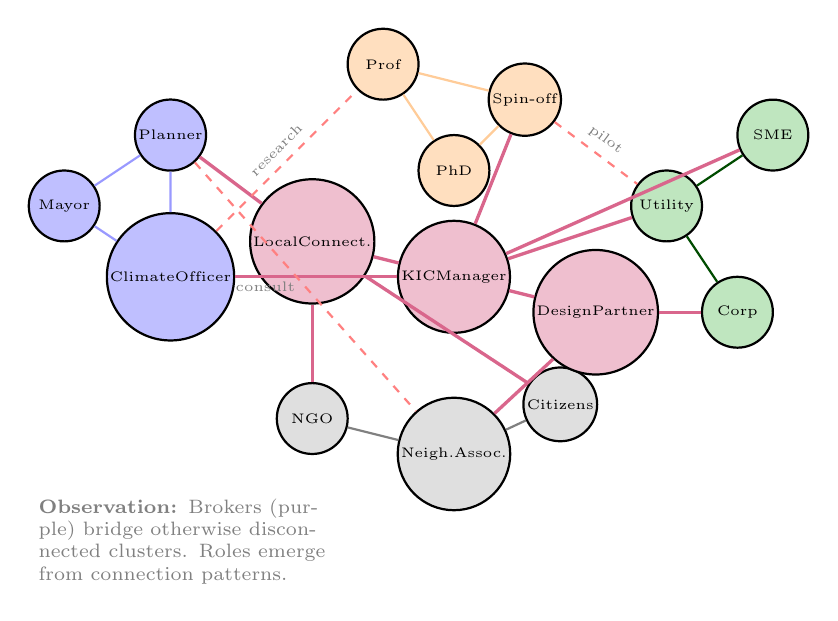
\begin{tikzpicture}[
    actor/.style={circle, draw, thick, fill=#1!25, minimum size=0.9cm, font=\tiny, inner sep=1pt},
    tie/.style={-, thick, #1},
    label/.style={font=\tiny, #1},
    scale=0.9
]
% Actors - positioned to show connection patterns
% City government cluster
\node[actor=blue] (planner) at (-4,2) {Planner};
\node[actor=blue] (climate) at (-4,0) {Climate\\Officer};
\node[actor=blue] (mayor) at (-5.5,1) {Mayor};

% University cluster  
\node[actor=orange] (prof) at (-1,3) {Prof};
\node[actor=orange] (spinoff) at (1,2.5) {Spin-off};
\node[actor=orange] (phd) at (0,1.5) {PhD};

% Business cluster
\node[actor=green!60!black] (utility) at (3,1) {Utility};
\node[actor=green!60!black] (sme) at (4.5,2) {SME};
\node[actor=green!60!black] (corp) at (4,-0.5) {Corp};

% Citizens cluster
\node[actor=gray] (ngo) at (-2,-2) {NGO};
\node[actor=gray] (assoc) at (0,-2.5) {Neigh.\\Assoc.};
\node[actor=gray] (cit) at (1.5,-1.8) {Citizens};

% Intermediaries (emergent brokers)
\node[actor=purple] (kic) at (0,0) {KIC\\Manager};
\node[actor=purple] (connector) at (-2,0.5) {Local\\Connect.};
\node[actor=purple] (design) at (2,-0.5) {Design\\Partner};

% Intra-cluster ties (thin, same color)
\draw[tie=blue!40] (planner) -- (climate) -- (mayor) -- (planner);
\draw[tie=orange!40] (prof) -- (spinoff) -- (phd) -- (prof);
\draw[tie=green!30!black] (utility) -- (sme);
\draw[tie=green!30!black] (utility) -- (corp);
\draw[tie=gray] (ngo) -- (assoc) -- (cit);

% Cross-cluster ties via brokers (thick, purple)
\draw[tie=purple!60, very thick] (kic) -- (climate);
\draw[tie=purple!60, very thick] (kic) -- (spinoff);
\draw[tie=purple!60, very thick] (kic) -- (utility);
\draw[tie=purple!60, very thick] (kic) -- (sme);

\draw[tie=purple!60, very thick] (connector) -- (planner);
\draw[tie=purple!60, very thick] (connector) -- (ngo);
\draw[tie=purple!60, very thick] (connector) -- (cit);
\draw[tie=purple!60, very thick] (connector) -- (kic);

\draw[tie=purple!60, very thick] (design) -- (assoc);
\draw[tie=purple!60, very thick] (design) -- (corp);
\draw[tie=purple!60, very thick] (design) -- (kic);

% Direct cross-cluster ties (dashed, emerging)
\draw[tie=red!50, dashed] (spinoff) -- (utility) node[midway, above, label=gray, sloped] {pilot};
\draw[tie=red!50, dashed] (climate) -- (prof) node[midway, above, label=gray, sloped] {research};
\draw[tie=red!50, dashed] (planner) -- (assoc) node[midway, left, label=gray] {consult};

% Annotation
\node[anchor=north west, font=\scriptsize, text width=4cm, gray] at (-6,-3) {
    \textbf{Observation:} Brokers (purple) bridge otherwise disconnected clusters. Roles emerge from connection patterns.
};
\end{tikzpicture}
\caption{Ground-level actor connections in a Deep Demonstration site. Cluster structure and brokerage positions visible before role labels assigned.}
\label{fig:local-ties}
\end{figure}

%% ============================================
%% FIGURE 8: Constellation Motifs
%% ============================================
\begin{figure}[htbp]
\centering
\begin{tikzpicture}[
    node/.style={circle, draw, thick, fill=#1!30, minimum size=0.7cm, font=\scriptsize},
    inter/.style={circle, draw=purple, very thick, fill=purple!25, minimum size=0.7cm, font=\scriptsize},
    tie/.style={-, thick},
    motifbox/.style={rectangle, rounded corners, draw=gray!50, dashed, minimum width=3.2cm, minimum height=2.8cm},
    scale=0.85
]
% Motif A: Mediated Triad
\node[motifbox] at (0,0) {};
\node[font=\small\bfseries] at (0,1.7) {A: Mediated Triad};
\node[node=blue] (a1) at (-0.8,0.5) {A};
\node[inter] (ai) at (0,-0.3) {I};
\node[node=green!60!black] (a2) at (0.8,0.5) {B};
\draw[tie] (a1) -- (ai) -- (a2);
\node[font=\tiny, gray] at (0,-1.1) {I brokers A--B};

% Motif B: Knowledge Triangle
\node[motifbox] at (4,0) {};
\node[font=\small\bfseries] at (4,1.7) {B: Knowledge Triangle};
\node[node=blue] (b1) at (3.2,0.6) {U};
\node[node=orange] (b2) at (4.8,0.6) {R};
\node[node=green!60!black] (b3) at (4,-0.5) {B};
\node[inter] (bi) at (4,0.2) {I};
\draw[tie] (b1) -- (b2) -- (b3) -- (b1);
\draw[tie, purple!60] (bi) -- (b1);
\draw[tie, purple!60] (bi) -- (b2);
\draw[tie, purple!60] (bi) -- (b3);
\node[font=\tiny, gray] at (4,-1.1) {Closed U-R-B triad};

% Motif C: Legitimacy Bridge
\node[motifbox] at (8,0) {};
\node[font=\small\bfseries] at (8,1.7) {C: Legitimacy Bridge};
\node[node=green!60!black, minimum size=0.9cm] (c1) at (7.2,0.5) {Corp};
\node[inter] (ci) at (8,0) {I};
\node[node=teal, minimum size=0.5cm] (c2) at (8.8,0.5) {Start};
\draw[tie, very thick] (c1) -- (ci) -- (c2);
\draw[-Stealth, red!50, thick, bend left=30] (c1) to node[above, font=\tiny] {legitimacy} (c2);
\draw[-Stealth, blue!50, thick, bend left=30] (c2) to node[below, font=\tiny] {innovation} (c1);
\node[font=\tiny, gray] at (8,-1.1) {Bidirectional transfer};

% Motif D: Demonstration Cluster
\node[motifbox, minimum width=3.5cm, minimum height=3cm] at (12,0) {};
\node[font=\small\bfseries] at (12,1.8) {D: Demo Cluster};
\node[node=blue, minimum size=0.9cm] (d0) at (12,0.3) {Place};
\node[node=teal, minimum size=0.4cm] (d1) at (10.8,0.8) {};
\node[node=teal, minimum size=0.4cm] (d2) at (11.2,-0.5) {};
\node[node=teal, minimum size=0.4cm] (d3) at (12.5,-0.7) {};
\node[node=orange, minimum size=0.5cm] (d4) at (13.2,0.6) {Reg};
\draw[tie, teal!60] (d0) -- (d1);
\draw[tie, teal!60] (d0) -- (d2);
\draw[tie, teal!60] (d0) -- (d3);
\draw[tie, orange!60, very thick] (d0) -- (d4);
\node[font=\tiny, gray] at (12,-1.2) {Niche-regime interface};

% Legend
\node[font=\tiny, gray, anchor=west] at (-1.5,-2.2) {U=University, R=Research, B=Business, I=Intermediary, Corp=Corporate, Start=Start-up, Reg=Regime actor};
\end{tikzpicture}
\caption{Recurring constellation motifs discovered across EIT demonstration sites}
\label{fig:motifs}
\end{figure}

%% ============================================
%% FIGURE 9: Bottom-Up Emergence of Multi-Level Structure
%% ============================================
\begin{figure}[htbp]
\centering
\begin{tikzpicture}[
    local/.style={circle, draw, fill=#1!25, minimum size=0.25cm, inner sep=0pt},
    hub/.style={ellipse, draw=teal, thick, fill=teal!15, minimum width=1.4cm, minimum height=0.9cm, font=\tiny},
    kic/.style={ellipse, draw=purple, very thick, fill=purple!20, minimum width=1.8cm, minimum height=1cm, font=\scriptsize\bfseries},
    eit/.style={rectangle, rounded corners, draw=gray, very thick, fill=gray!15, minimum width=2cm, minimum height=0.8cm, font=\small\bfseries},
    cluster/.style={ellipse, draw=gray, dashed, minimum width=2.2cm, minimum height=1.6cm},
    agg/.style={-Stealth, thick, gray!60, dashed},
    tie/.style={-, thin, gray!40},
    scale=0.7
]
% Level labels
\node[font=\small\bfseries, rotate=90, anchor=south] at (-7,0) {Emergence};
\draw[-Stealth, very thick, gray] (-6.5,-3) -- (-6.5,4.5);

% Ground level - scattered local actors
\node[font=\scriptsize, anchor=east] at (-5.5,-2.5) {Local ties};
\foreach \x in {-4,-2.5,-1,0.5,2,3.5,5} {
    \foreach \y in {-3,-2.2} {
        \pgfmathsetmacro{\r}{random(1,4)}
        \ifnum\r=1 \node[local=blue] at (\x+rand*0.3,\y+rand*0.2) {}; \fi
        \ifnum\r=2 \node[local=orange] at (\x+rand*0.3,\y+rand*0.2) {}; \fi
        \ifnum\r=3 \node[local=green!60!black] at (\x+rand*0.3,\y+rand*0.2) {}; \fi
        \ifnum\r=4 \node[local=purple] at (\x+rand*0.3,\y+rand*0.2) {}; \fi
    }
}

% Demo clusters emerge
\node[font=\scriptsize, anchor=east] at (-5.5,-0.5) {Clusters};
\node[cluster] (c1) at (-3,-0.5) {};
\node[font=\tiny] at (-3,-0.5) {Leuven};
\node[cluster] (c2) at (0,-0.5) {};
\node[font=\tiny] at (0,-0.5) {Milan};
\node[cluster] (c3) at (3,-0.5) {};
\node[font=\tiny] at (3,-0.5) {Madrid};
\node[cluster] (c4) at (5.5,-0.5) {};
\node[font=\tiny] at (5.5,-0.5) {Vejle};

% Aggregation arrows level 1
\draw[agg] (-3.5,-2) -- (-3,-1.3);
\draw[agg] (-0.5,-2) -- (0,-1.3);
\draw[agg] (2.5,-2) -- (3,-1.3);
\draw[agg] (5,-2) -- (5.5,-1.3);

% Hub level
\node[font=\scriptsize, anchor=east] at (-5.5,1.5) {Hubs};
\node[hub] (h1) at (-1.5,1.5) {DACH/\\Benelux};
\node[hub] (h2) at (1.5,1.5) {Iberia/\\Italy};
\node[hub] (h3) at (4.5,1.5) {Nordic};

% Aggregation arrows level 2
\draw[agg] (c1) -- (h1);
\draw[agg] (c2) -- (h2);
\draw[agg] (c3) -- (h2);
\draw[agg] (c4) -- (h3);

% Cross-hub bridges
\draw[tie, thick, purple!50] (h1) -- (h2);
\draw[tie, thick, purple!50] (h2) -- (h3);

% KIC level
\node[font=\scriptsize, anchor=east] at (-5.5,3.2) {KIC};
\node[kic] (kic) at (1.5,3.2) {Climate-KIC};

% Aggregation arrows level 3
\draw[agg] (h1) -- (kic);
\draw[agg] (h2) -- (kic);
\draw[agg] (h3) -- (kic);

% EIT level
\node[font=\scriptsize, anchor=east] at (-5.5,4.5) {EIT};
\node[eit] (eit) at (1.5,4.5) {EIT};
\draw[agg] (kic) -- (eit);

% Annotation
\node[anchor=north west, font=\tiny, text width=5cm, gray] at (6.5,0) {
    \textbf{Key insight:} Multi-level structure emerges from aggregation of local connection patterns, not top-down design. Each level crystallises when coordination demands exceed capacity of level below.
};
\end{tikzpicture}
\caption{Bottom-up emergence: local ties $\rightarrow$ demonstration clusters $\rightarrow$ regional hubs $\rightarrow$ KIC $\rightarrow$ EIT}
\label{fig:bottom-up-emergence}
\end{figure}

%% ============================================
%% FIGURE 10: Role-Connection Duality
%% ============================================
\begin{figure}[htbp]
\centering
\begin{tikzpicture}[
    actor/.style={circle, draw, thick, minimum size=1.1cm, font=\tiny, inner sep=1pt},
    filled/.style={fill=#1!30},
    metric/.style={rectangle, rounded corners, draw=gray, fill=gray!5, minimum width=2.2cm, minimum height=0.6cm, font=\tiny},
    arr/.style={-Stealth, thick},
    scale=0.85
]
% Left side: Connection pattern
\node[font=\small\bfseries] at (-4,3) {Observed Connections};

\node[actor, filled=purple] (a) at (-4,1.5) {Actor\\X};
\node[actor, filled=blue] (b1) at (-6,0) {B1};
\node[actor, filled=blue] (b2) at (-5.2,0.8) {B2};
\node[actor, filled=orange] (c1) at (-2,0) {C1};
\node[actor, filled=orange] (c2) at (-2.8,0.8) {C2};
\node[actor, filled=green!60!black] (d1) at (-4,-1) {D1};

% Connections
\draw[thick] (a) -- (b1);
\draw[thick] (a) -- (b2);
\draw[thick] (a) -- (c1);
\draw[thick] (a) -- (c2);
\draw[thick] (a) -- (d1);
\draw[thin, gray] (b1) -- (b2);
\draw[thin, gray] (c1) -- (c2);

% Structural metrics
\node[font=\small\bfseries] at (0,3) {Structural Position};
\node[metric] at (0,2) {Degree: 5};
\node[metric] at (0,1.2) {Betweenness: High};
\node[metric] at (0,0.4) {Bridges clusters: 3};
\node[metric] at (0,-0.4) {Constraint: Low};

% Arrow
\draw[arr, very thick] (-1.5,1) -- (1.5,1);
\node[font=\tiny, anchor=south] at (0,1.1) {compute};

% Right side: Emergent role
\node[font=\small\bfseries] at (4,3) {Emergent Role};

\node[actor, filled=purple, minimum size=1.8cm] (role) at (4,0.5) {\textbf{Orchestrator}};

% Role characteristics
\node[font=\tiny, anchor=west, text width=3cm] at (5.5,1.5) {$\bullet$ Bridges disconnected groups};
\node[font=\tiny, anchor=west, text width=3cm] at (5.5,1) {$\bullet$ Low redundancy in ties};
\node[font=\tiny, anchor=west, text width=3cm] at (5.5,0.5) {$\bullet$ Information control};
\node[font=\tiny, anchor=west, text width=3cm] at (5.5,0) {$\bullet$ Coordination capacity};

% Arrow
\draw[arr, very thick] (1.8,0.5) -- (2.8,0.5);
\node[font=\tiny, anchor=south] at (2.3,0.6) {infer};

% Bottom annotation
\node[anchor=north, font=\scriptsize, text width=10cm, align=center, gray] at (0,-2) {
    \textbf{Role-connection duality:} The ``orchestrator'' role is not a label but a structural position defined by bridging connections. The role \textit{is} the connection pattern.
};
\end{tikzpicture}
\caption{Role-connection duality: roles inferred from structural position, not assigned \textit{a priori}}
\label{fig:role-connection}
\end{figure}

\subsection{Theoretical Contributions}

The bottom-up analysis of EIT constellations yields five propositions for role constellation theory:

\begin{enumerate}[noitemsep,topsep=2pt]
    \item \textbf{Roles emerge from connections.} Structural position in the network determines role, not formal designation. An actor ``becomes'' an orchestrator by accumulating bridging ties (Figure~\ref{fig:role-connection}).
    
    \item \textbf{Constellations exhibit motif recurrence.} Certain micro-structures (mediated triads, knowledge triangles, legitimacy bridges) appear repeatedly across sites, suggesting structural regularities amenable to pattern discovery.
    
    \item \textbf{Multi-level structure is emergent.} The EIT hierarchy (local $\rightarrow$ hub $\rightarrow$ KIC $\rightarrow$ EIT) crystallised from accumulated local connections, not top-down design. Each level emerges when coordination demands exceed lower-level capacity.
    
    \item \textbf{Intermediaries are constellation architects.} Systemic intermediaries do not merely occupy bridging positions---they actively cultivate constellation configurations through portfolio design, partner selection, and certification practices.
    
    \item \textbf{Constellation dynamics follow connection dynamics.} As ties form and dissolve (e.g., through funding cycles), role distributions shift. Tracking connection changes predicts role reconfigurations.
\end{enumerate}

This bottom-up perspective reframes role constellations not as static typologies but as \textit{emergent relational configurations}---patterns discovered through systematic observation of who connects to whom, and how those connections aggregate into recognizable structures.